\documentclass{standalone}
\begin{document}
\subsection{Segmentation}

The metric used for checking the performance of the segmentation results is given by the Dice Similarity Coefficient (DSC) evaluated on the validation set.
This is because it was the most used in literature for this purpose and so for make it possible results comparison.
The total number of involved patients lowered from 48 to 37 because of misregistration between images and medical annotations for some of them.
The training process was performed for 150 epochs\footnote{The term epoch indicates the number of passes of the entire training dataset the machine learning algorithm has completed.} on 391 images (training set) and validated on 97 images (validation set).
The Training process took almost 7 hours, on the new Apple Silicon M1 Macbook Pro equipped with 8 GB of RAM.
The results of the training process can be seen in Figure \ref{training}.
The plots show the curves for the model dice coefficient and the model loss as a function of the epochs.
In particular, the blue curve represents the results obtained for the training set of data while the green one represents the results obtained for the validation set.
\\
In Table \ref{results}, you can see the comparison between the state of the art and the implemented pipeline about colorectal cancer segmentation.
We must remember that the literature about MRI colorectal cancer segmentation performed by using CNNs, unlike other topics, is not very wide.
However, it comes out that automatic segmentation is quite hard to perform on Magnetic Resonance colorectal cancer images due to different issues: data; medical annotations; loss function.
In fact, as showed by Jovana Panic at al.\cite{jpanic} mucinous cases can considerably affect the performances.
Moreover, the performance can be affected by how medical annotations are made.
Trebeschi et al. \cite{Trebeschi2017} showed that the DSC of the same model trained using medical annotations made by different experts can give different DSC scores.
Another sensitive factor is the loss function. 
As shown by Yi. Jie Huang et al.\cite{YiJieHuang}, depending on the network's architectures and the loss functions you can have different performances. 
 
\begin{table}[ht]
	\Large
	\centering
	\resizebox{\textwidth}{!}{\begin{tabular}{p{4.8cm}p{4.6cm}p{4.9cm}p{5cm}p{4.9cm}} \toprule
		{\textbf{Trebeschi et al.}} & {\textbf{Panic et al.}} & {\textbf{Yi-Jie Huang et al.}} & {\textbf{Xiaoling Pang et al.}} & {\textbf{Implemented pipeline}} \\ \midrule
		DSC= 0.68  & DSC = 0.58   &  DSC = $[0.66 - 0.72]$  &  DSC = 0.66 &  \textbf{DSC = 0.71} \\
		DSC= 0.70&   &  & &   \\
		\midrule
		140 patients &  33 patients & 64 cancerous cases & 275 patients & \textbf{37 patients}  \\
			& (5 mucinous cases)  &  & excluding mucinous  & \textbf{including some }  \\
			&   &  & cases  & \textbf{mucinous cases}    \\
	\midrule
	Custom Network  &   Custom Network  & Custom network  & U-net & \textbf{U-net, backbone} \\
	architecture & architecture  &  architectures &   &  \textbf{EfficientNetb0}  \\
	\bottomrule
	\end{tabular}}

	\caption{Results comparison between state-of-art and the implemented pipeline about MRI colorectal cancer scans segmentation by using CNNs.}
	\label{results}
	
\end{table}


\begin{figure}[ht]

    \centering
    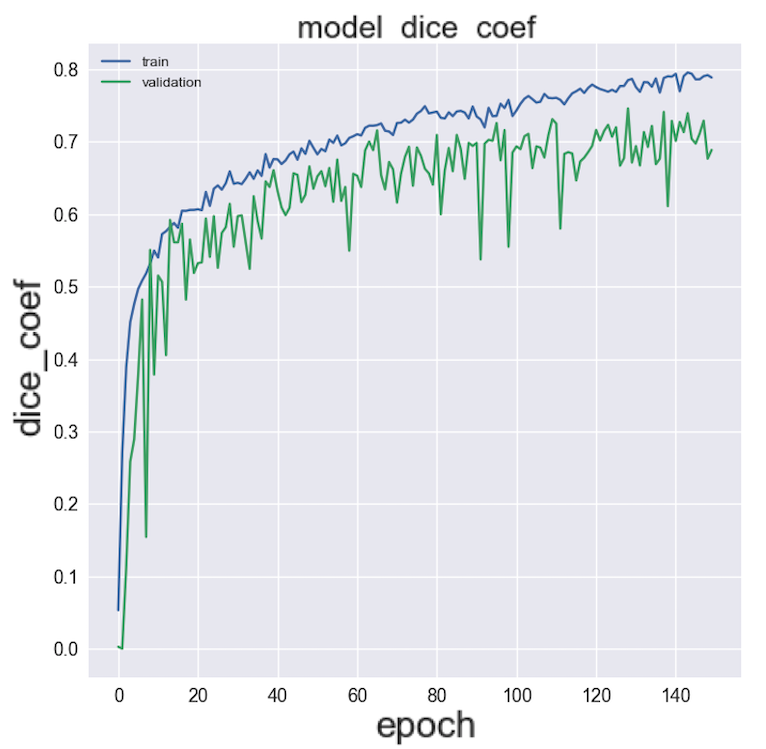
\includegraphics[width=0.49\textwidth]{../images/dice_coef.png}
	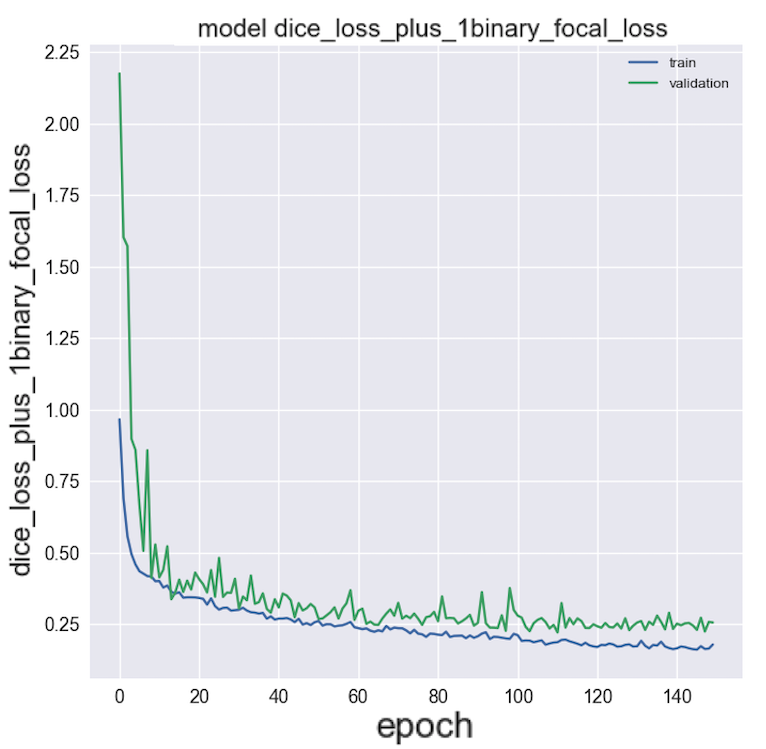
\includegraphics[width=0.49\textwidth]{../images/loss.png}

    \caption{Model history plots on training (blue) and validation (green) set. \textit{Left}): DSC as a function of the epochs. \textit{Right}): model loss as a function of the epochs.}
    \label{training}
    
\end{figure}
\clearpage
\newpage

\subsubsection{Comparison with Manual Annotations}


To check the pipeline performances, I have also compared the obtained segmentation with the manual annotation (Ground-truth) made by expert radiologists.
In Figure \ref{predtraining}, you can see the comparison for images belonging to the training set while in Figure \ref{predvalidation} the comparison for the ones belonging to the validation set.
The prediction is plotted as a probability density map between 0. and 1. as shown by the sequential colormap.
Both in Figure \ref{predtraining} and \ref{predvalidation}, I also included a case of \textit{mucinous} (first row), showing that the model is able to distinguish also this type of tumor, even if the contour is not as precise as the ground-truth one.
\\
Unfortunately, for a few cases, the model failed to segment correctly the right Region of Interest (ROI).
Some of this cases are shown in Figure \ref{predwrong}.
\\
The goodness of the comparison can also be appreciated from the comparison between the ground truth and the prediction over the original image.
In Figure \ref{predoverlaptraining} and \ref{predoverlaptraining2} the images belong to the training set while in Figure \ref{predoverlapvalidation} and \ref{predoverlapvalidation2} the images belong to the validation one.
Also for this case, the prediction is plotted as a probability density map between 0. and 1. as shown by the sequential colormap.


\begin{figure}[htp]

    \centering
    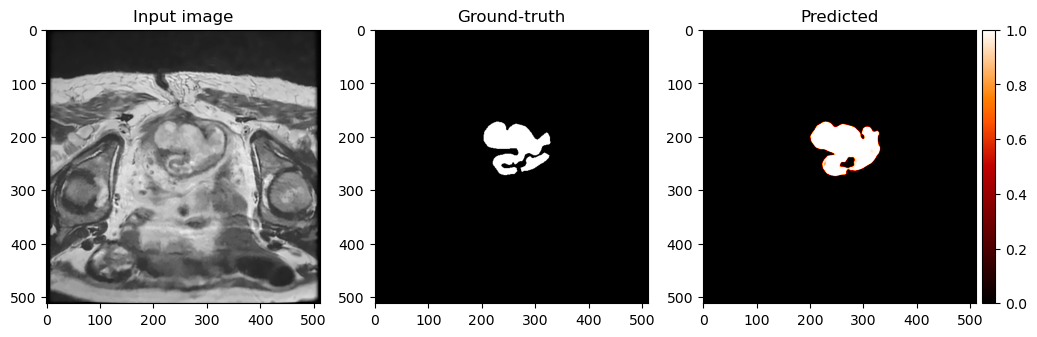
\includegraphics[width=\textwidth]{../images/predoutputr.png}
    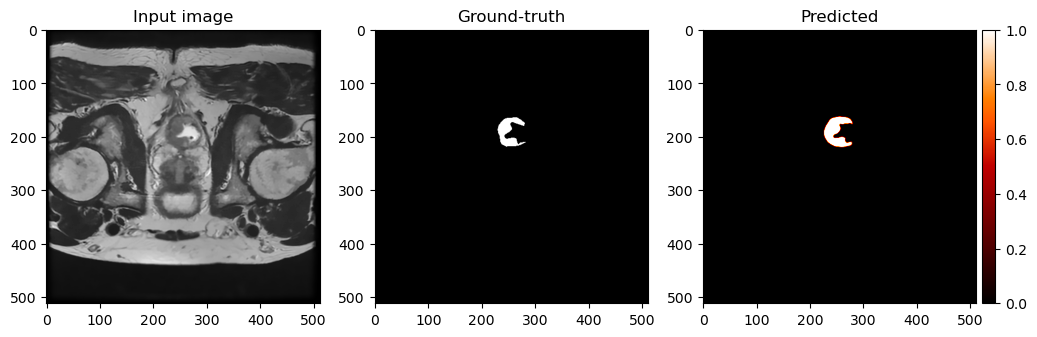
\includegraphics[width=\textwidth]{../images/predoutputr1.png}
    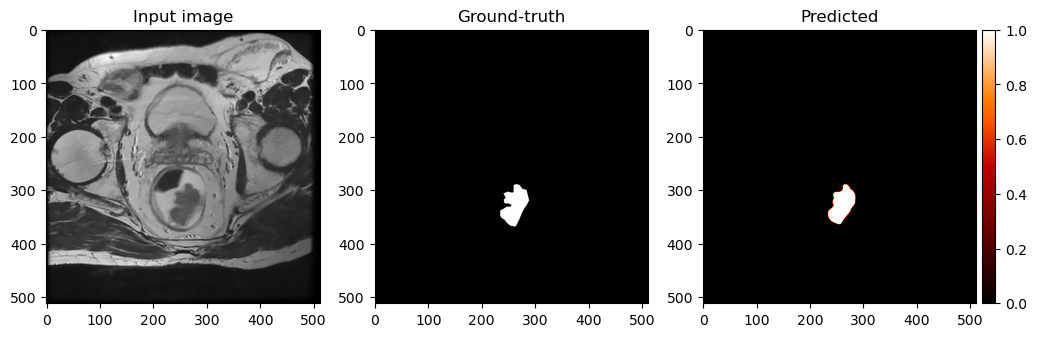
\includegraphics[width=\textwidth]{../images/predoutputr2.png}

    \caption{Comparison between the ground-truth image and the predicted one by the CNN model. The first column represents the input image. 
    The second one represents the ground-truth image. 
    Finally, the third one represents the predicted tumor area.
    The prediction is plotted as a probability density map between 0. and 1. as shown by the sequential colormap.
    From training set.}\label{predtraining}


\end{figure}



\begin{figure}[htp]

    \centering
    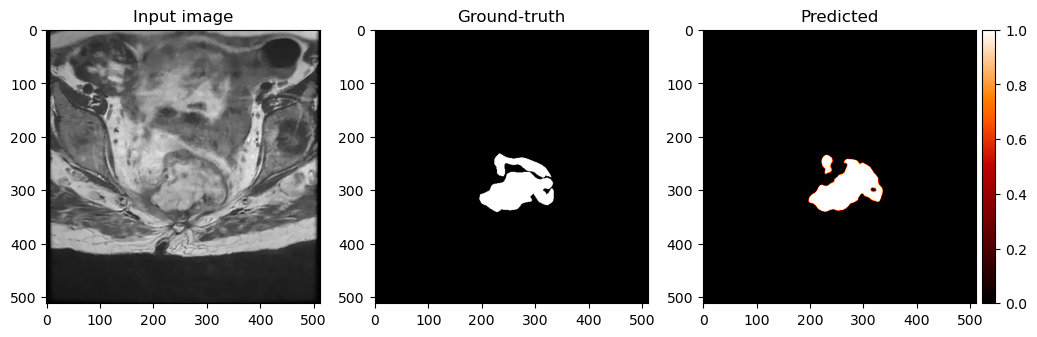
\includegraphics[width=\textwidth]{../images/predoutput2.png}
    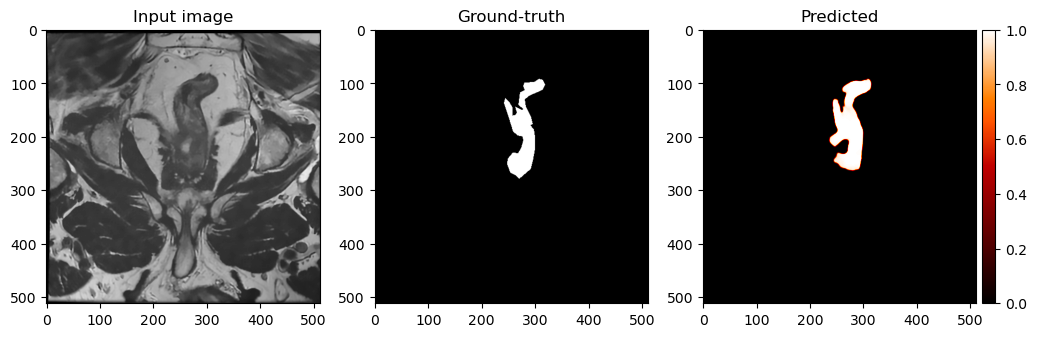
\includegraphics[width=\textwidth]{../images/predoutput.png}
    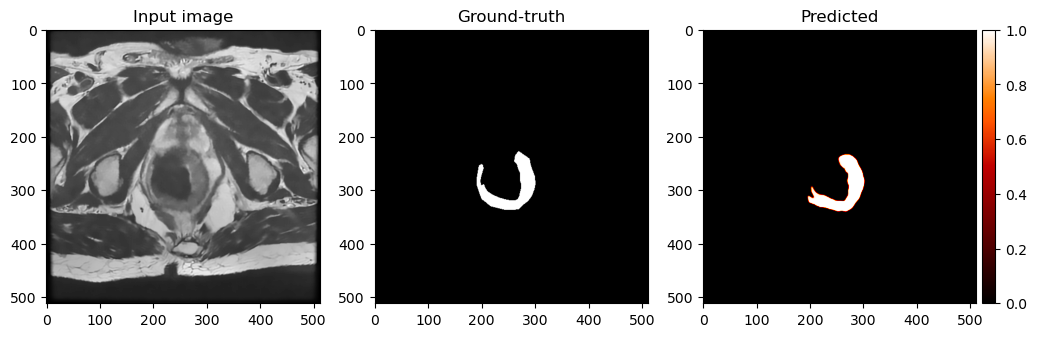
\includegraphics[width=\textwidth]{../images/predoutput1.png}
    

    \caption{Comparison between the ground-truth image and the predicted one by the CNN model. The first column represents the input image. 
    The second one represents the ground-truth image. 
    Finally, the third one represents the predicted tumor area.
    The prediction is plotted as a probability density map between 0. and 1. as shown by the sequential colormap.
    From validation set.}\label{predvalidation}

\end{figure}


\begin{figure}[htp]

    \centering
    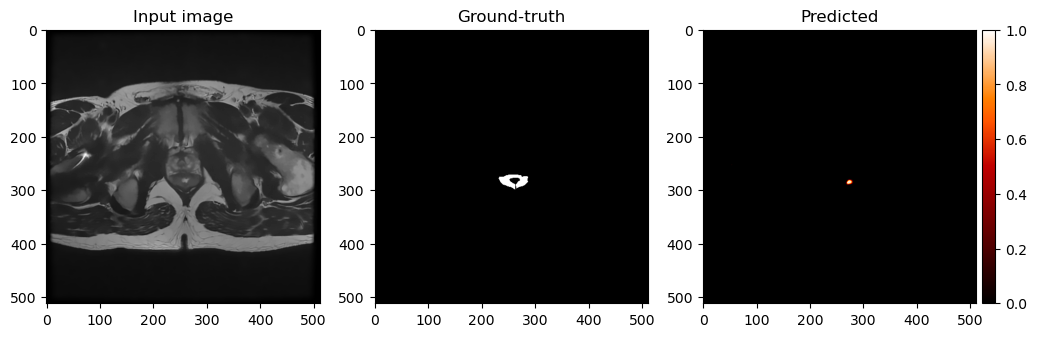
\includegraphics[width=\textwidth]{../images/predoutputwrong.png}
    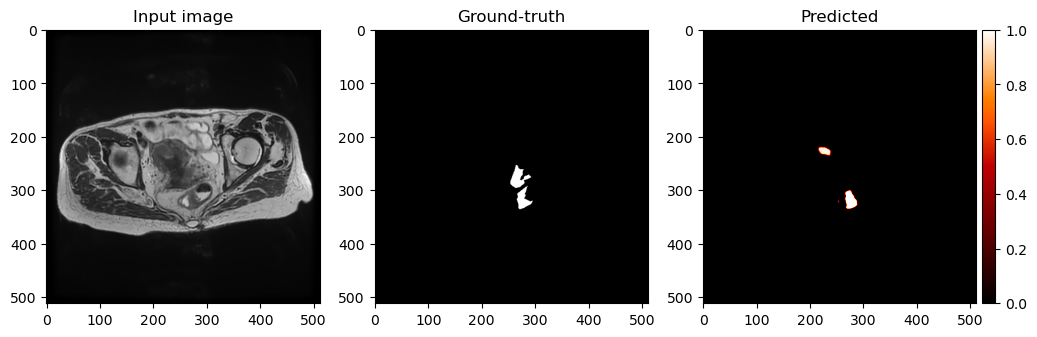
\includegraphics[width=\textwidth]{../images/predoutputwrong1.png}
    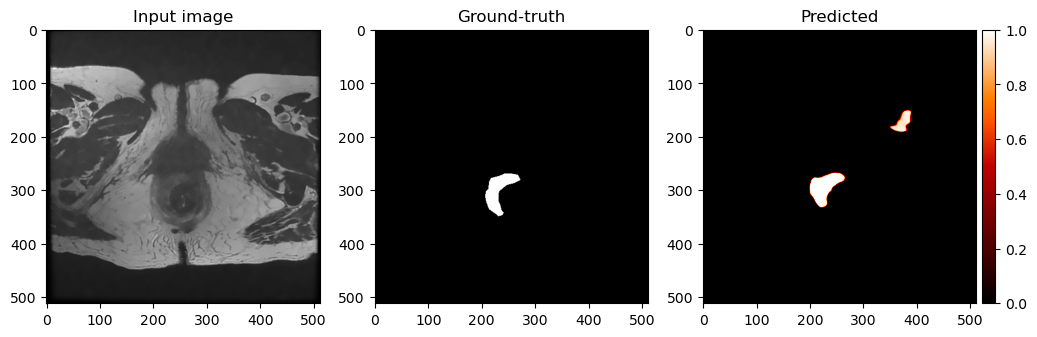
\includegraphics[width=\textwidth]{../images/predoutputwrong2.png}
    

    \caption{Comparison between the ground-truth image and the predicted one by the CNN model. The first column represents the input image. 
    The second one represents the ground-truth image. 
    Finally, the third one represents the predicted tumor area.
    The prediction is plotted as a probability density map between 0. and 1. as shown by the sequential colormap.
    Bad segmentation cases.}\label{predwrong}

\end{figure}


\begin{figure}[htp]

    \centering
    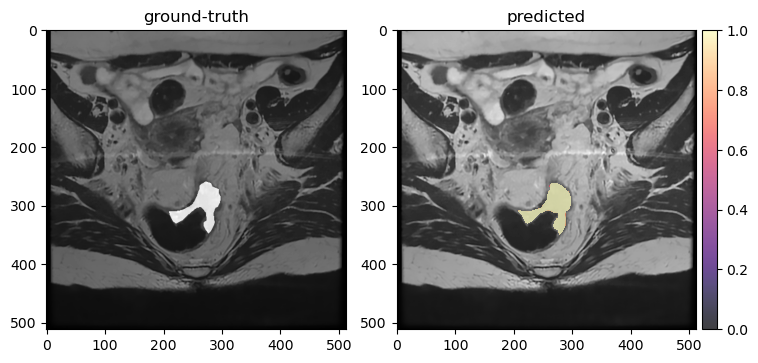
\includegraphics[width=\textwidth]{../images/predoutputoverlap2.png}
    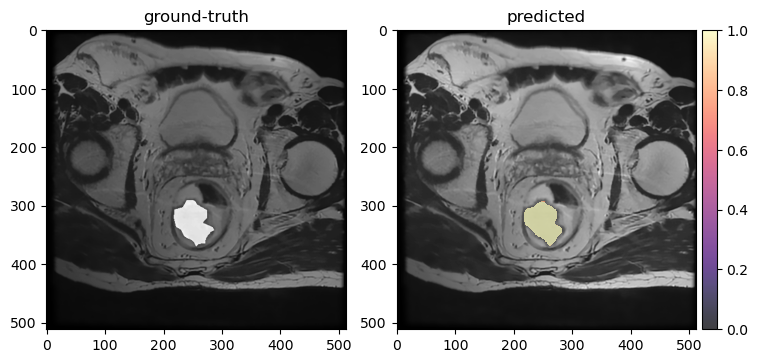
\includegraphics[width=\textwidth]{../images/predoutputoverlap1.png}
    
    \caption{Comparison between the ground-truth image and the prediction over the original image.
    The prediction is plotted as a probability density map between 0. and 1. as shown by the sequential colormap.
    From training set.}\label{predoverlaptraining}

\end{figure}

\begin{figure}[htp]

    \centering
    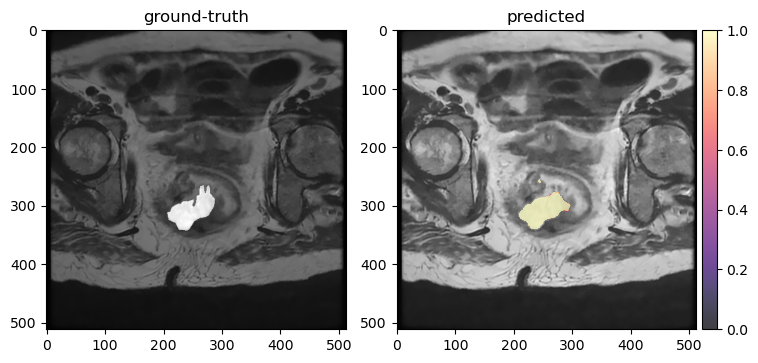
\includegraphics[width=\textwidth]{../images/predoutputoverlap3.png}
    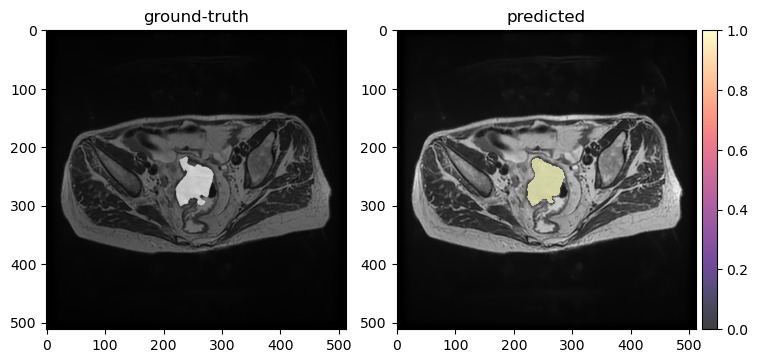
\includegraphics[width=\textwidth]{../images/predoutputoverlap4.png}
    
    \caption{Comparison between the ground-truth image and the prediction over the original image.
    The prediction is plotted as a probability density map between 0. and 1. as shown by the sequential colormap.
    From training set.}\label{predoverlaptraining2}

\end{figure}

\begin{figure}[htp]

    \centering
    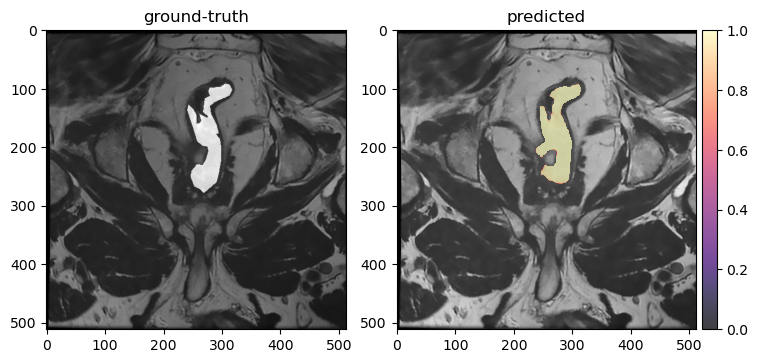
\includegraphics[width=\textwidth]{../images/predoutputoverlapvalidation.png}
    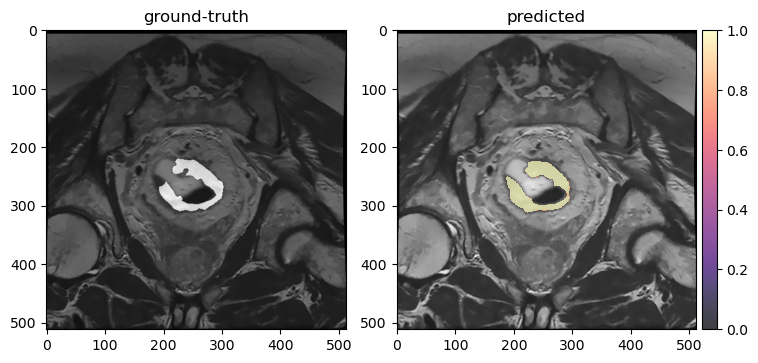
\includegraphics[width=\textwidth]{../images/predoutputoverlapvalidation1.png}
    
    
    \caption{Comparison between the ground-truth image and the prediction over the original image.
    The prediction is plotted as a probability density map between 0. and 1. as shown by the sequential colormap.
    From validation set.}\label{predoverlapvalidation}

\end{figure}


\begin{figure}[htp]

    \centering
    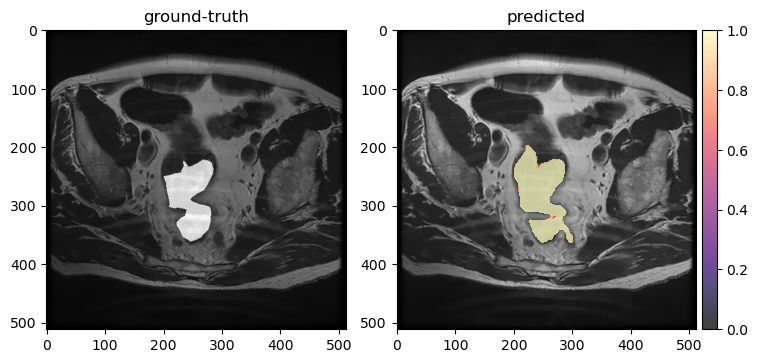
\includegraphics[width=\textwidth]{../images/predoutputoverlapvalidation2.png}
    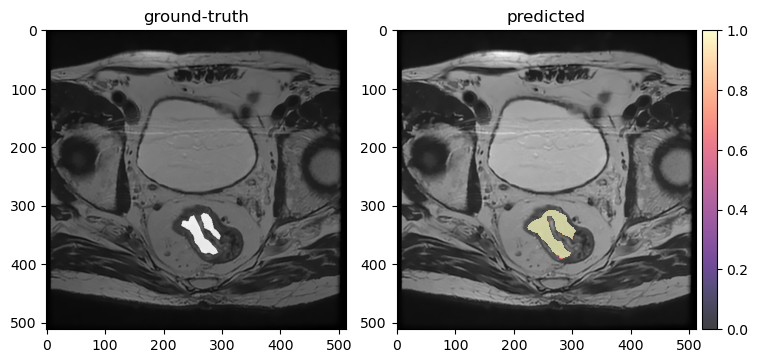
\includegraphics[width=\textwidth]{../images/predoutputoverlapvalidation3.png}
    
    
    \caption{Comparison between the ground-truth image and the prediction over the original image.
    The prediction is plotted as a probability density map between 0. and 1. as shown by the sequential colormap.
    From validation set.}\label{predoverlapvalidation2}

\end{figure}


\newpage
\end{document}